\section{Hasil dan Pembahasan}
\subsection{Pemeliharaan Struktur Dokumen}
Tabel~\ref{tab:chunking} menunjukkan bahwa \tech{structure-aware chunker} menghasilkan \tech{recall} tertinggi dalam kedua perbandingan pada $K=25$. Pada \tech{User Manual}, selisihnya terhadap \tech{recursive} adalah 0,130 dan terhadap \tech{sliding-window} adalah 0,065. Pada peraturan, selisihnya masing-masing 0,04 dan 0,03.

\begin{table}[tb]
\centering\small
\caption{\tech{Recall} perbandingan \tech{chunker}, $K=25$.}
\label{tab:chunking}
\begin{tabularx}{\columnwidth}{@{}>{\RaggedRight\arraybackslash}Xrr@{}}
\toprule
Strategi & \tech{User Manual} & Peraturan\\\midrule
\tech{Structure-aware} & \textbf{0,740} & \textbf{0,64}\\
\tech{Recursive} & 0,610 & 0,60\\
\tech{Sliding-window} & 0,675 & 0,61\\\bottomrule
\end{tabularx}
\smallskip
\parbox{\columnwidth}{\footnotesize Strategi peraturan menggunakan varian \tech{legal structure-aware}. \tech{Indexer} dibuat tetap dalam setiap korpus, yaitu \tech{hybrid} untuk \tech{User Manual} dan \tech{dense} untuk peraturan.}
\end{table}

Hasil tersebut konsisten dengan manfaat mempertahankan hubungan \tech{block} dan konteks induknya pada manual, serta batas pasal dan ayat pada peraturan. Namun, perbandingan ini menguji konfigurasi lengkap setiap \tech{chunker}. Tanpa eksperimen tambahan yang menghilangkan konteks induk secara terpisah, seluruh selisih tidak dapat diatribusikan hanya pada satu mekanisme struktural.

\subsection{Pencarian pada \tech{User Manual}}
Pada $K=40$, \tech{dense indexer} mencapai \tech{recall} gabungan 0,830. Nilainya adalah 0,850 untuk pertanyaan bahasa Inggris dan 0,810 untuk bahasa Indonesia. Selisih empat poin persentase menunjukkan bahwa pencarian berbasis representasi semantik tetap menemukan sebagian besar referensi ketika bahasa pertanyaan berbeda dari bahasa dokumen.

Untuk membandingkan kondisi pada jumlah kandidat yang sama, Tabel~\ref{tab:manual} menggunakan $K=45$. \tech{Dense} mencapai 0,835, lebih tinggi daripada \tech{hybrid baseline} sebesar 0,745 dan \tech{sparse} sebesar 0,465. \tech{Recursive} dan \tech{sliding-window} pada tabel ini tetap menggunakan \tech{hybrid indexer}.

\begin{table}[tb]
\centering\small
\caption{Hasil \tech{User Manual} pada $K=45$.}
\label{tab:manual}
\begin{tabularx}{\columnwidth}{@{}>{\RaggedRight\arraybackslash}Xrrr@{}}
\toprule
Kondisi & \tech{Recall} & \tech{Precision} & \tech{nDCG}\\\midrule
\tech{Hybrid baseline} & 0,745 & 0,033 & 0,339\\
\tech{Recursive} & 0,630 & 0,022 & 0,294\\
\tech{Sliding-window} & 0,685 & 0,028 & 0,325\\
\tech{Sparse} & 0,465 & 0,023 & 0,177\\
\tech{Dense} & \textbf{0,835} & \textbf{0,045} & \textbf{0,380}\\\bottomrule
\end{tabularx}
\end{table}

Pertanyaan mengenai gejala dan prosedur dapat memakai parafrasa yang tidak muncul secara literal dalam manual. Karena itu, hasil \tech{dense} sesuai dengan kebutuhan pencarian berdasarkan makna. Penambahan jalur pencocokan istilah pada \tech{hybrid} belum tentu membantu setiap pertanyaan, terutama pada pencarian lintas bahasa. Gambar~\ref{fig:manual} memperlihatkan hubungan cakupan pencarian dengan jumlah kandidat.

\begin{figure*}[t]
\centering
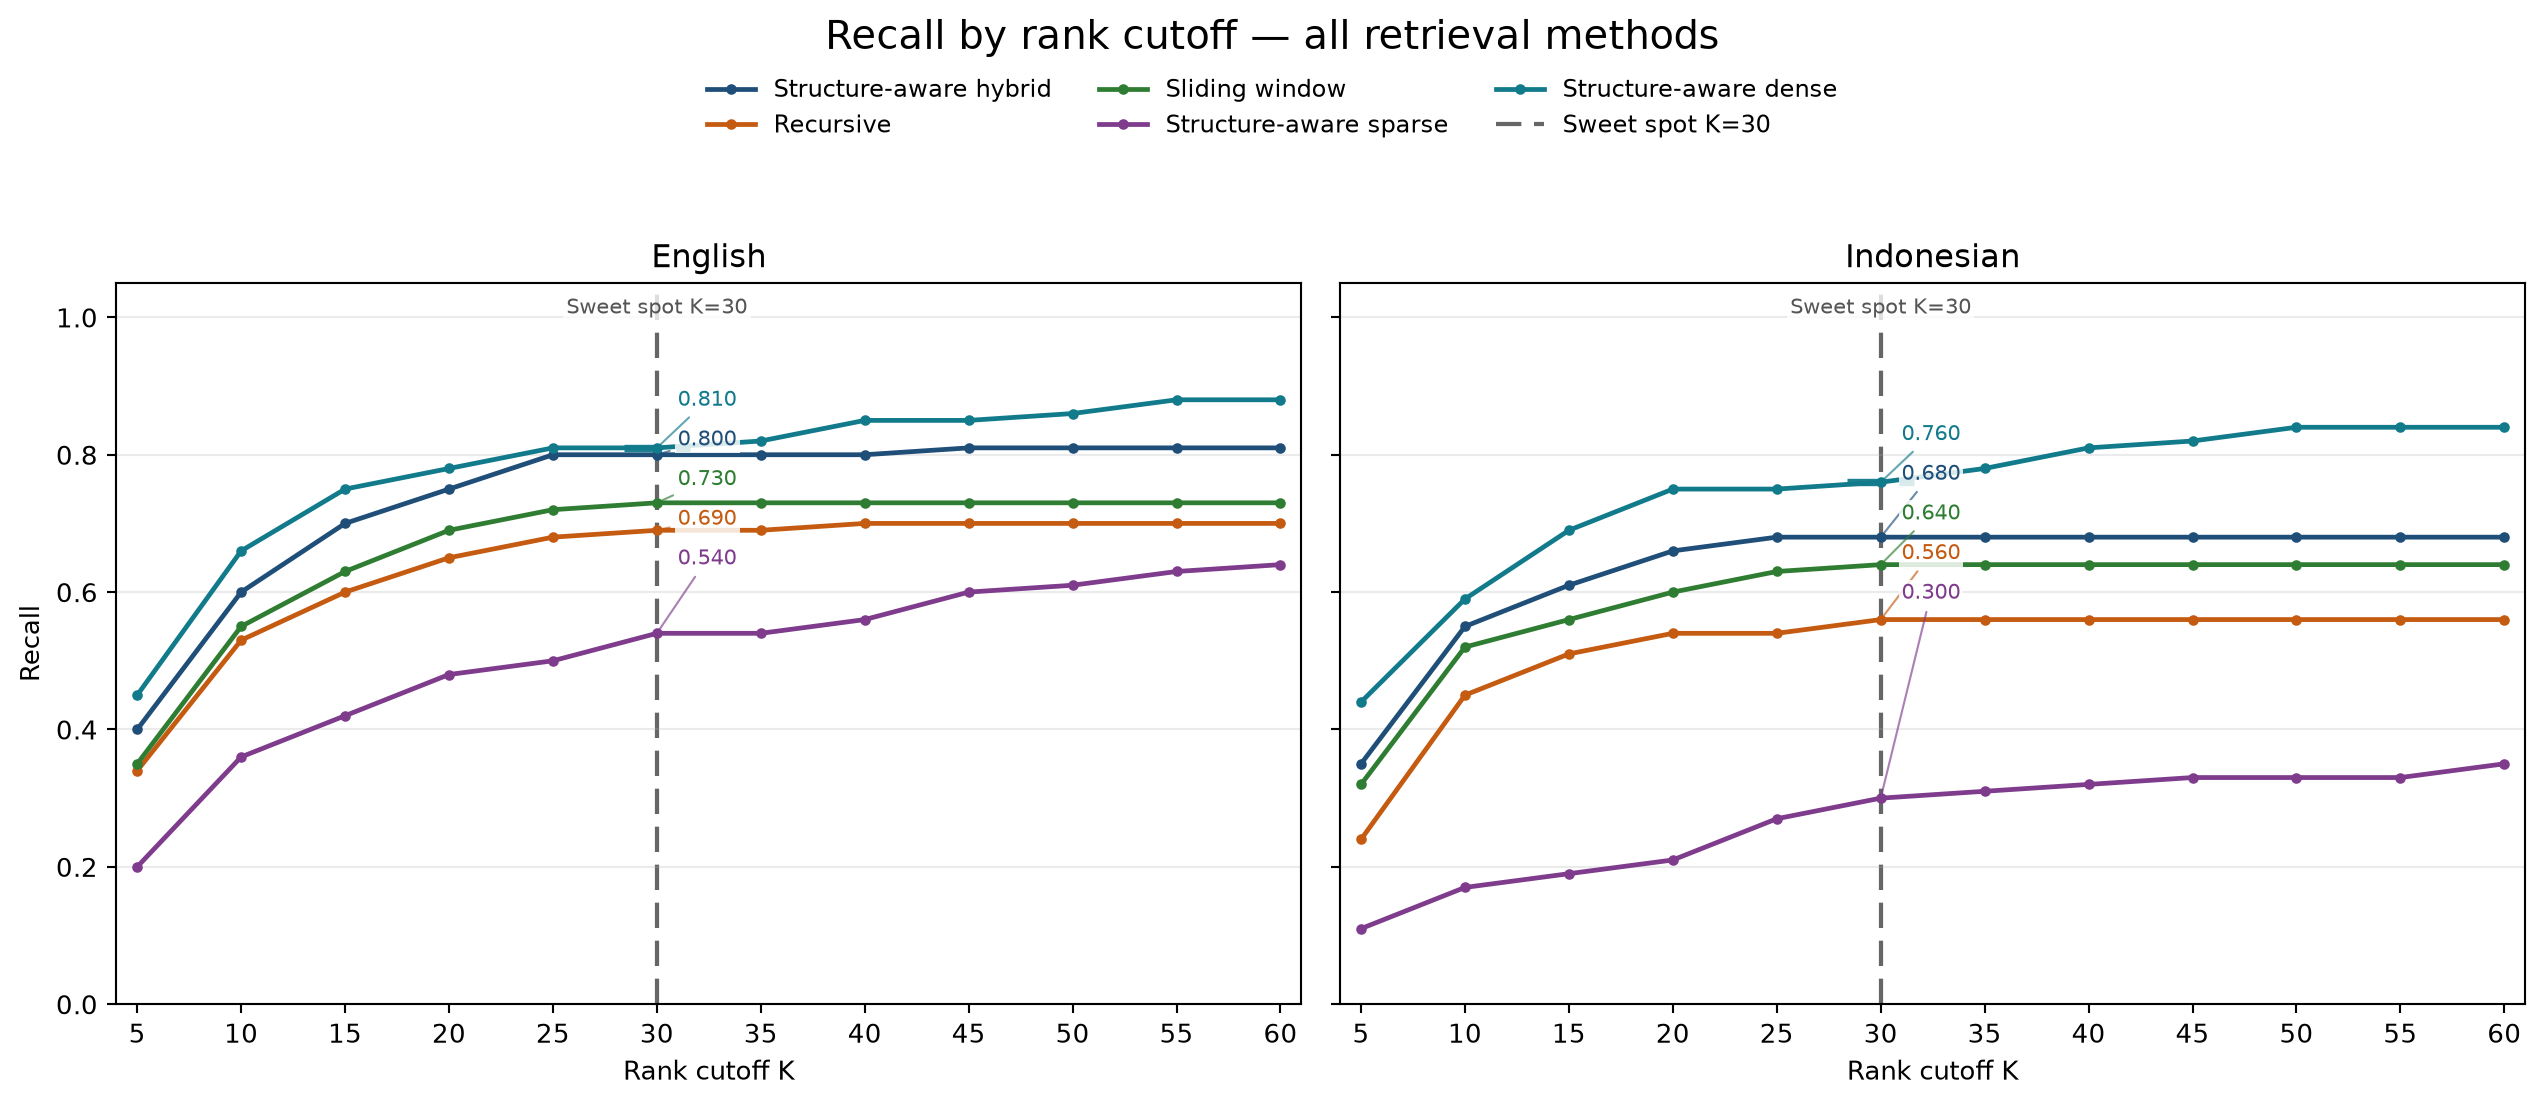
\includegraphics[width=0.9\textwidth]{../src/images/experiments/customer_service_revision/final_eda/recall-all-retrieval.png}
\caption{\tech{Recall} pada \tech{User Manual} untuk berbagai nilai $K$.}
\label{fig:manual}
\end{figure*}

\subsection{Pencarian pada Peraturan}
Pada pemilihan model dengan $K=45$, BAAI/BGE-M3 mencapai \tech{recall} 0,65, sedangkan Indo-LegalBERT mencapai 0,45. Hasil ini mendasari penggunaan BAAI/BGE-M3 sebagai model acuan pada perbandingan komponen berikutnya. Temuan tersebut terbatas pada konfigurasi dan pertanyaan yang digunakan.

Pada $K=25$, \tech{hybrid indexer} memperoleh \tech{recall} tertinggi sebesar 0,67, sedangkan \tech{dense} dan \tech{sparse} sama-sama mencapai 0,64 (Tabel~\ref{tab:legal}). Pertanyaan hukum dapat menggabungkan istilah atau identitas peraturan yang eksplisit dengan uraian kebutuhan informasi. Kombinasi pencocokan istilah dan makna memberikan cakupan lebih tinggi pada korpus ini.

\begin{table}[tb]
\centering\small
\caption{Hasil peraturan pada $K=25$.}
\label{tab:legal}
\begin{tabularx}{\columnwidth}{@{}>{\RaggedRight\arraybackslash}Xrrr@{}}
\toprule
Kondisi & \tech{Recall} & \tech{Precision} & \tech{nDCG}\\\midrule
\tech{Dense baseline} & 0,64 & 0,047 & \textbf{0,445}\\
Indo-LegalBERT & 0,43 & 0,025 & 0,203\\
\tech{Recursive} & 0,60 & 0,038 & 0,381\\
\tech{Sliding-window} & 0,61 & 0,040 & 0,407\\
\tech{Sparse} & 0,64 & \textbf{0,071} & 0,358\\
\tech{Hybrid} & \textbf{0,67} & 0,068 & 0,437\\\bottomrule
\end{tabularx}
\end{table}

Keunggulan \tech{recall} tidak berarti seluruh ukuran ikut tertinggi. \tech{Sparse} menghasilkan \tech{precision} 0,071, sedangkan \tech{dense} menghasilkan \tech{nDCG} 0,445. Pemilihan \tech{hybrid} mengikuti tujuan menemukan referensi sebanyak mungkin sebelum tahap \tech{downstream}. Nilai \tech{precision} yang rendah juga memperlihatkan bahwa kandidat masih mengandung banyak bagian yang tidak relevan. Peningkatan kualitas jawaban setelah \tech{reranking} belum diuji.

\subsection{Penelusuran Hubungan dalam Graf}
Pada 30 pertanyaan relasi dan $K=25$, \tech{sparse} menghasilkan \tech{KG recall} 0,517, diikuti \tech{hybrid} 0,417, \tech{sliding-window} 0,350, serta \tech{dense baseline} dan \tech{recursive} masing-masing 0,300. Penggantian model ke Indo-LegalBERT menghasilkan 0,150. Gambar~\ref{fig:kg} menampilkan perubahan ukuran ini terhadap $K$.

\begin{figure*}[t]
\centering
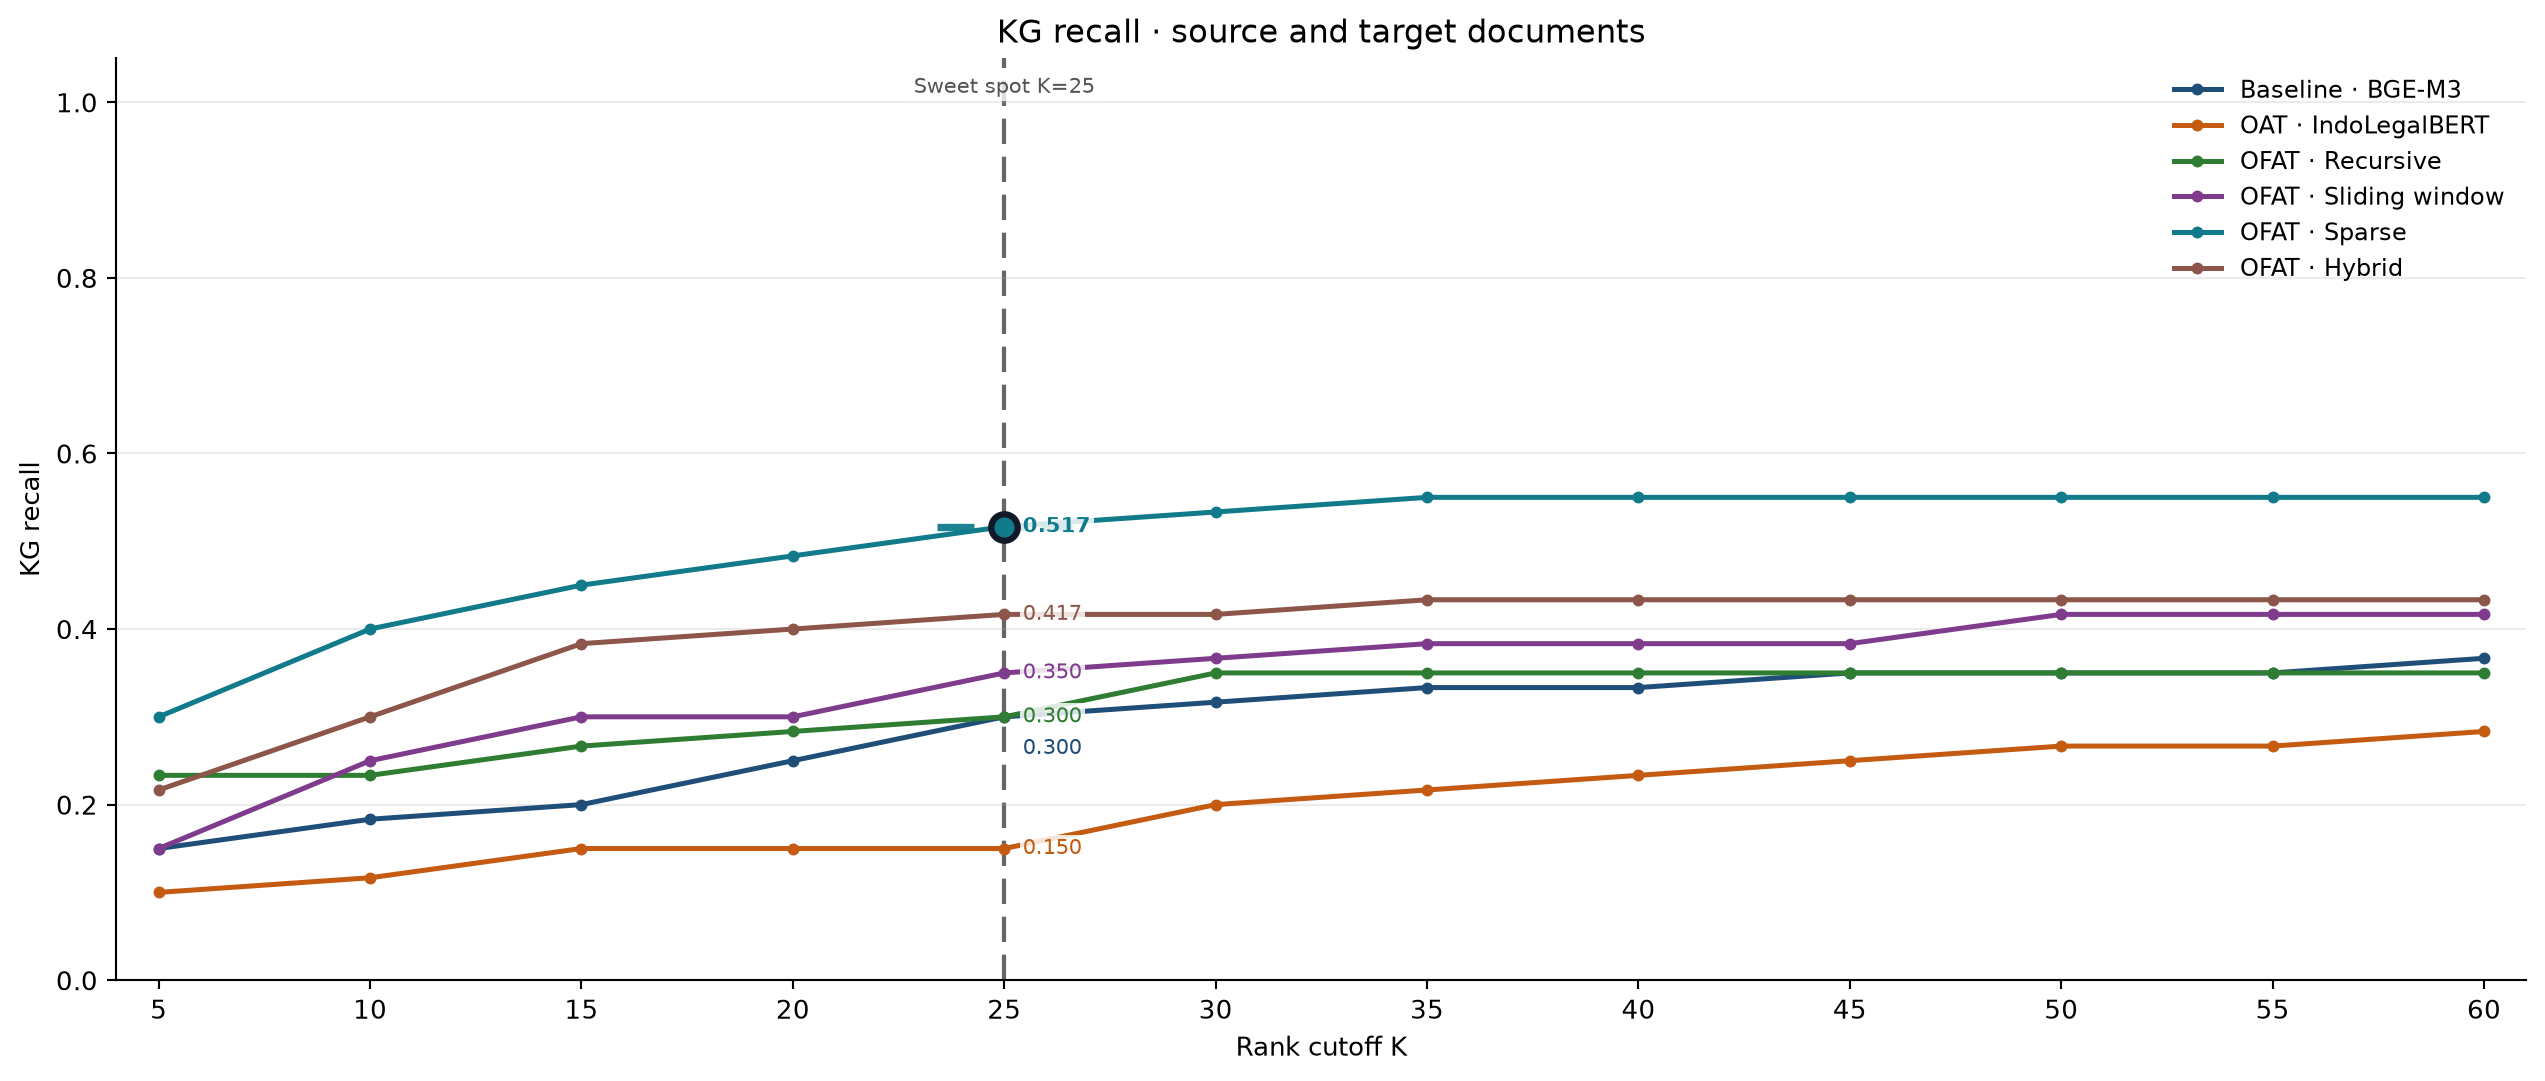
\includegraphics[width=0.9\textwidth]{../src/images/experiments/legal_revision/final_eda/kg-recall-all-retrieval.png}
\caption{\tech{KG recall} pada pertanyaan relasi peraturan.}
\label{fig:kg}
\end{figure*}

Keunggulan \tech{sparse} pada kelompok ini konsisten dengan pertanyaan yang menyebut entitas atau penanda peraturan secara eksplisit. Hasilnya tidak bertentangan dengan keunggulan \tech{hybrid} pada keseluruhan pertanyaan karena cakupan evaluasinya berbeda. Evaluasi ini merupakan diagnostik penelusuran relasi pada korpus peraturan. Tidak tersedia hasil kuantitatif pembanding graf pada \tech{User Manual} dalam eksperimen yang dirangkum.

\subsection{Implikasi dan Keterbatasan}
Arsitektur \tech{plugin} menyediakan tempat untuk menerapkan strategi yang berbeda tanpa mengubah kontrak informasi. Pada dua korpus ini, pemeliharaan struktur memberi hasil \tech{chunking} terbaik, tetapi strategi pencarian terpilih berbeda. Oleh karena itu, perluasan \tech{domain} perlu disertai evaluasi konfigurasi, bukan sekadar penggunaan ulang konfigurasi lama.

Angka antarkorpus tidak dapat dibaca sebagai perbandingan langsung tingkat kesulitan. Korpus, jumlah referensi acuan, bahasa, dan nilai $K$ berbeda. Pasangan pertanyaan dualbahasa juga berbagi konteks, sementara pertanyaan hukum dari PSU yang sama berbagi sumber. Jumlah pertanyaan karena itu tidak sama dengan jumlah observasi yang sepenuhnya independen.

Pemilihan peraturan hanya mencakup dokumen yang siap diproses secara vektor. Manual terbatas pada sembilan produk Netgear. Pertanyaan disusun dengan bantuan model dari konteks acuan, sehingga belum tentu mencerminkan distribusi pertanyaan pengguna nyata. OFAT belum menguji interaksi antarkomponen, dan tidak ada klaim signifikansi statistik atas selisih hasil. Pengukuran kualitas jawaban, biaya operasional, keamanan, dan efektivitas komponen percakapan memerlukan evaluasi tersendiri.
